\section{Noise}

Noise is one of the most fundamental concepts of PCG and there exists several flavors of it.
The two major types of noise are \textit{value noise} and \textit{gradient noise}, which can both be expressed using the following function.
$$
  f(\vec x) = y \in [0, 1] \text{ where }
  y \in \mathbb{R},
  \vec x \in \mathbb{R}^n,
  n \in \mathbb{Z}^+
$$
This function is deterministic, but the output for any single input is perceived as random.
This is achieved by combining a Random Number Generator (RNG) with an interpolation function.
The way that these two functions are implemented and utilized is what differs value noise from gradient noise.

Value noise is constructed by first randomizing the values of all lattice points in an $n$-dimensional space using an RNG function.
These points are then interpolated to define intermediate points, resulting in a continuous $n$-dimensional space of random values.
The noise function then simply outputs the real number defined at coordinate $\vec x$ within this space.
The interpolation function used is typically bilinear or bicubic in the setting of real-time computer graphics, as they are computationally cheap.

Although simple to implement, value noise has several disadvantages.
First off, the resulting noise has a visually grid-like structure.
This is often undesired in graphics since it creates arbitrary patterns in the noise.
Moreover, neighboring lattice points sometimes greatly differ in values which can result in sudden changes in intensity.

Gradient noise solves the major problems present in value noise by randomizing $n$-dimensional gradient vectors at each lattice point, instead of real numbers.
This modification ensures that the interpolated values have smooth continuous gradients (i.e. partial derivatives) and not just smoothly interpolated values.

Some common implementations of gradient noise include \textit{Perlin noise} \cite{perlin_noise} \cite{perlin_noise2}, \textit{Simplex noise} \cite{simplex_noise}, and \textit{OpenSimplex noise} \cite{opensimplex_noise_blog} \cite{opensimplex_noise_code}.
Ken Perlin originally invented Perlin noise with the intention to produce more natural-looking textures \cite{perlin_noise}, and later invented Simplex noise to address some of the limitations with Perlin noise \cite{simplex_noise}.
Usage of Simplex noise is however restricted due to its patent \cite{opensimplex_noise_patent}.
Fortunately, Kurt Spencer invented a well-performing variation called \textit{OpenSimplex noise} which was released into the public domain \cite{opensimplex_noise_blog} \cite{opensimplex_noise_code}.
The details of these algorithms are beyond the scope of this paper, but further reading of Perlin noise can be found in the original paper \cite{perlin_noise}, and the ideas behind Simplex noise are described in great detail by Stefan Gustavson in his paper \textit{Simplex noise demystified} \cite{simplex_noise_explained}.

In practice, it is common to use a Fractional Brownian Motion (fBm) implementation, which can be constructed by summing noise functions of different amplitudes and sampling frequencies.
The variation in frequency and the variation in amplitude between these functions are sometimes referred to as lacunarity and gain respectively.
The usage of fBm allows for greater control over the resulting noise function's visual properties, making it more suitable for many applications in computer graphics.

\begin{figure}[h!]
  \centering
  \begin{subfigure}[b]{0.30\textwidth}
    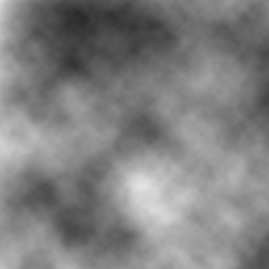
\includegraphics[width=\textwidth]{figure/value_noise.png}
    \caption{Value noise. \cite{value_noise_img}}
  \end{subfigure}
  \quad
  \quad
  \quad
  \begin{subfigure}[b]{0.30\textwidth}
    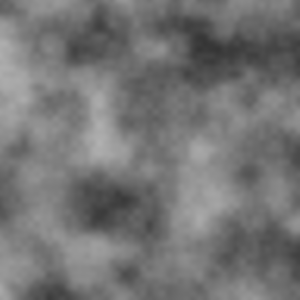
\includegraphics[width=\textwidth]{figure/perlin_noise.png}
    \caption{Gradient noise. \cite{perlin_noise_img}}
  \end{subfigure}

  \caption{Examples of value noise and gradient noise represented using intensity maps. Notice how the value noise has cross-like patterns.}
  \label{fig:noisetypes}
\end{figure}

The output of noise functions can be visualized in many ways, intensity maps being one of them (see figure~\ref{fig:noisetypes}).
An intensity map is a bitmap image where each pixel represents the value of the underlying noise.
Bright pixels represent high values, while dark pixels represent low values.
These maps can be used to represent various things such as heights, in which case they are referred to as \textit{heightmaps}.
They can also be used to blend textures together, which is called \textit{texture splatting}.